\documentclass[0-thesis.tex]{subfiles}

\begin{document}
This thesis proposes an update architecture based on SUIT. The architecture is technology
agnostic and adds on top of SUIT tokens and certificates for identifying and authorizing
actors, a life cycle perspective on device management, and defines what information is
needed for a device to take part of an update procedure. Furthermore the thesis presents
profiles for the architecture which implementers can use, these are introduced in Chapter
\ref{chap:profiles}. Five key areas that the architecture must define have been
identified:

\begin{itemize}
    \item Roles of devices, servers, and operators
    \item Key management of IoT update procedure
    \item Device profiles and communication
    \item Update authorization
    \item Update handling for local upgrades
\end{itemize}

\begin{figure}
    \caption{Example workflow of an update procedure.}
    \label{fig:communication-workflow}
    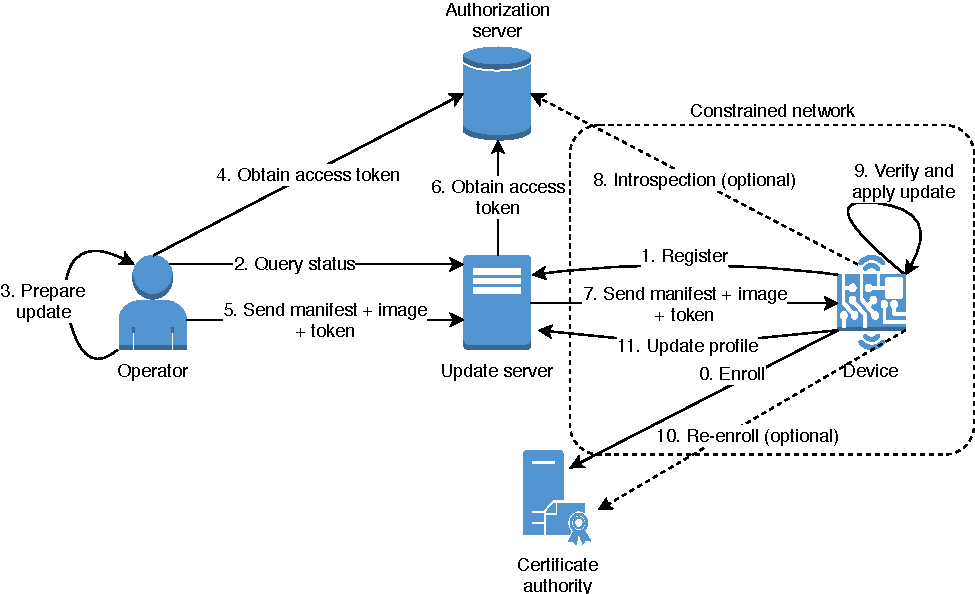
\includegraphics{images/update-flow.pdf}
\end{figure}

By putting the five key areas together, Figure~\ref{fig:communication-workflow} shows an
example update flow in the architecture. Note that where the SUIT standard would
differentiate between the author of an update and an operators, this architecture will for
simplicity regard them as the same entity, the operator. For the same reason, the
architecture will not differentiate between device and network operators. An operator is
an entity that tracks device statuses and prepares, signs, and sends updates to devices.
Figure~\ref{fig:communication-workflow} gives a brief introduction to the concepts needed
to understand the architecture, these concepts will be explained in more detail throughout
sections \ref{sec:roles}-\ref{sec:upgrading}. In this particular example the update
procedure is initiated by the operator by querying the update server for device status and
then pushing an update. The manifest and image are distributed together. The steps can be
briefly explained as:

\begin{enumerate}
    \setcounter{enumi}{-1}
    \item The \textbf{device} enrolls at the \textbf{CA} and receives a
            \textbf{certificate}.
    \item The device registers at the \textbf{update server} which creates a \textbf{profile}
            for the device.
    \item The \textbf{operator} queries the update server for device status in order to
            prepare an update.
    \item The operator prepares a \textbf{manifest} and \textbf{image} and signs them.
    \item The operator requests an \textbf{authorization token} from the
            \textbf{authorization server} in order to gain access to applying the update.
    \item The signed manifest and image are sent to the update server with the
            authorization token.
    \item The update server requests an authorization token from the authorization server
            in order to gain access to applying the update.
    \item The signed manifest and image are sent with the update server's authorization
            token to the device.
    \item The device requests introspection data from the authorization server to verify
            the authorization token. This step is optional.
    \item The device decrypts and verifies the manifest and image and applies the update.
    \item The device's certificate broke as part of the update and it uses a new
            pre-shared key included in the updated image to re-enroll. This step is
            optional.
    \item The device updates its profile at the update server by re-registering.
\end{enumerate}

Section~\ref{sec:roles} defines what a device, update server, and operator means in the
context of the update architecture. Section~\ref{sec:key-management} discusses what is
needed for devices to enroll in a PKI and how keys are handled during updates.
Section~\ref{sec:communication} describes how devices, update servers, and operators can
communicate and shows an example workflow of communicating an update.
Section~\ref{sec:authorization} describes the purpose of issuing authorization tokens, how
devices can use them, and who is to be authorized. Section~\ref{sec:upgrading} discusses
different means of handling the payload when applying an update.
Section~\ref{sec:manifest-format} introduces the manifest format proposed by the
architecture. Finally Section~\ref{sec:use-cases-examples-topologies} shows the
architecture applied to different use cases.

\section{Roles of Devices, Update Servers, and Operators}
\label{sec:roles}
This section explains the notion of devices, update servers, and operators in the
architecture, their responsibilities, and their intended functionality.
Section~\ref{ssec:what-is-a-device} briefly covers devices,
Section~\ref{ssec:what-is-an-update-server} covers the topic of update servers, and
Section~\ref{ssec:what-is-an-operator} covers operators.

\subsection{What Is a Device and What Do They Do?}
\label{ssec:what-is-a-device}
Devices are constrained, low-power IoT appliances connected to a constrained network. They
are running the applications of the network and performs simple tasks such as measurement
using sensors. The devices communicate wirelessly and must be secured from attackers while
being able to be updated. They communicate with each other, update servers, and operators.

Devices have to trust update servers and operators wanting to send them updates. In order
to do so, devices need predetermined whitelists of update servers and operators. The
identity of an update server or operator can be checked using certificates and by then
matching against the whitelists, communication can be allowed or prohibited. Update
servers and operators that are whitelisted still need to be authorized to perform an
update, this is discussed further in Section~\ref{sec:authorization}.

Communication with update servers and operators requires the update servers and operators
know how to reach the devices if they want to initiate contact. Devices must thus register
profiles at the update servers, and must be enrolled in order to be trusted. In order to
register a profile at an update server, the update server must offer an API that allows a
device to POST its information (vendor and class ID as well as version) to the update
server. How communication is handled and a further explanation of profiles is in
Section~\ref{sec:communication}.

To properly handle updates a device needs to implement a local update handler. The update
handler is responsible for decrypting manifests and images, parsing and verifying the
manifest, and preparing the image for boot. How and where the device stores manifest and
image is discussed in further detail in Section~\ref{sec:upgrading}.

\subsection{What Is an Update Server and What Do They Do?}
\label{ssec:what-is-an-update-server}
Update servers are responsible for transporting manifests and images to the devices,
acting as image repositories, and keeping track of device profiles. After enrollment
devices register at an update server and the update server creates a profile for that
device. The profile contains the vendor and class IDs and firmware version of the device.
This allows the update server to know through which protocols the device can be contacted
and which version it should be updated to. Operators, discussed in the next section, send
signed manifests and images to update servers, and can query them for device status.

Devices must contain a list of update servers and by trusting the certificate authority
they can verify update server certificates. An update server is thus any machine that is
enrolled, has a valid certificate, and is included in the device's list of update servers.
The reasoning behind this definition is that a standard solution for updates should not
assume the topology of an IoT network. The update server may be a machine acting as a
proxy between a traditional network containing the operator and a constrained network with
IoT devices. The update server could be a more capable IoT device located entirely within
the constrained network and be contacted through a proxy. The update server could be
located entirely within the traditional network and use a proxy to communicate with
devices of the constrained network. Section~\ref{sec:use-cases-examples-topologies} shows
different use cases, highlighting this aspect.

An update server must provide an API for a device to register, this can be done by letting
the device POST vendor and class IDs and version to some registration endpoint.
Furthermore devices must be able to pull updates from the update server, this also
requires some API the device can use for querying. The querying could be a GET request
from the device upon which the update server matches the profile of the device with
available manifests. The update server should offload the device as much as possible when
it comes to picking an update as devices will typically have much tougher energy
constraints. In addition, update servers act as repositories for updates and have much
more information regarding which update is suitable.

Additionally operators will also be querying the update server for statuses of devices.
This functionality can be more fleshed out as it interacts with a human being and can
offer filters for retrieving statuses of devices from a certain vendor or class, or
devices running a certain firmware version. Allowing the operator to filter devices in the
network while querying is important as IoT networks can contain a large amount of
different devices, and it is imperative to find the ones in critical need of updates
first.

A device can be aware of several update servers, and different devices can be mapped to
different update servers. Optionally, different devices can be mapped to different
endpoints of the same physical update server. This can make device management easier as
certain classes of devices can be handled by certain update servers. By allowing a device
to receive updates from several update servers, the update mechanism architecture also
displays a form of robustness. If one update server is for instance located entirely
within the constrained network and the connection between that update server and the
operator is severed, updates can still be distributed through other update servers. If
devices are pulling updates, they can query the update servers in order of their list of
update servers. If updates are pushed, devices keep the connection with the update server
pushing the update.

Which machines are allowed to act like update servers can be boiled down to a few
important points no matter the topology of choice:

\begin{itemize}
    \item An update server is enrolled and has a valid certificate
    \item An update server is included in a device's list of update servers
    \item An update server can request authorization tokens and be authorized to update a
            device
    \item An operator can reach the update server and is authorized by the update server
            to query device status and upload manifests and images
\end{itemize}

\subsection{What Is an Operator and What Do They Do?}
\label{ssec:what-is-an-operator}
% TODO: Operators need a way of creating manifests, querying update servers, and using the
% queried device profiles to send updates either directly or through the update server.
Operators are people authorized to upload manifests and images to an update server. They
can also optionally upload manifests directly to a device depending on the network
topology. Operators prepare manifests and images, signs and transports them with an
authorization token to an update server, which then forwards them to a device. The signing
ensures end-to-end security for images and manifests between operators and devices.
Authorization is further discussed in Section~\ref{sec:authorization}.

Like a list of update servers introduced in Section~\ref{ssec:what-is-a-device}, devices
also need a list of operators. This is because if an operator wishes to send a manifest
directly to a device, the device needs to be aware of the operator and permit traffic from
that operator. Just like with mapping devices to update servers, devices can receive
manifests from several operators and different devices may interact with different
operators. 

Mapping devices to different operators creates opportunities to logically divide a network
between operators. An example use case is a constrained network supported by different
vendors where the respective vendors should only be able to service their respective
devices. It can also create a hierarchy, where certain operators may directly interact
with devices but other operators must interact with devices through update servers. Yet
again the point is to prepare for as many different scenarios as possible and create a
flexible architecture.

Operators need a way of creating manifests in order to update devices. In order to create
a manifest they must be aware of which devices are going to be updated and what firmware
versions they are using. This information is held by the update server in form of device
profiles. An operator can query the update server selecting the devices of interest based
on vendor or class ID or possibly firmware version. 

As the manifest contains data difficult for humans to craft such as image hash digest and
sequence numbers possibly in the form of timestamps, operators should be able to provide
information such as manifest version, vendor and class IDs, firmware version, and URL to a
program which then generates, encodes, and signs the manifest for them. Such a program can
also sign the image and send the manifest and image without further intervention from the
operator, this is implementation specific. The point is operators need help from the
update server when deciding about which devices to update, and should be given help
filling in the details of the manifest to ensure its correctness.

As with update servers, the essence of being an operator can be captured in a few points:

\begin{itemize}
    \item An operator is enrolled and has a valid certificate
    \item An operator is included in a device's list of operators
    \item An operator can request authorization tokens and be authorized to update a
            device
    \item An operator is trusted by an update server to query device status and send
            manifests and images to the update server
\end{itemize}

\section{Key Management of IoT Update Procedure}
\label{sec:key-management}
% TODO: Consider updates breaking certificates. Why would they? Lack of understanding concerning
% certificates perhaps
% Two pairs of keys from one PSK? Are two pairs needed?
The architecture will, in order to align with the goals of SUIT, be based on asymmetric
cryptography. The availability of EST-coaps makes this feasible in IoT contexts but other
enrollment protocols could also be used. This means a \gls{ca} is needed to act as a
trusted third party distributing certificates. The certificates are linked to a public key
which has a private key partner and are used to verify the correctness of a public key.
Certificates are signed by the CA and in order to trust them, device have to trust the CA
itself.

In order to enroll, a pre-shared key is proposed. This is the approach used in EST-coaps,
but it is not chosen for that reason. If a pre-shared key is not used the CA cannot be
sure the device asking to enroll really should be part of the trusted network. If an
attacker obtains a valid certificate they could communicate with devices and update
servers alike and no one would be able to tell it is a malicious actor. CAs must know they
are issuing certificates to the correct devices and pre-shared keys gives devices a means
of identifying themselves. Pre-shared keys could be used for encrypting all traffic but as
they are less scalable and harder to manage than certificates, they are just used for
enrolling.

A device that is enrolling has to trust the CA issuing the certificate. If it cannot do
so, how could it know it received a valid certificate? An attacker would love for a device
to use the attacker's public key instead, and if an attacker poses as a CA it could issue
a certificate with its own public key and then sign it. In order to trust the CA, a device
needs to have the certificate of the CA it is enrolling with or some other CA further down
the chain of trust. By verifying the signature on the newly enrolled certificate with the
CAs own certificate, a device can be certain they are using the correct keys.

There are options concerning how many key pairs a device should have. Device-to-device
communication might occur in the constrained network depending on the applications running
and it would also require asymmetric cryptography for identification. Devices receiving
updates might communicate with update servers or operators outside the constrained
network. If the same key pair is used for device-to-device communication and updates and
an attacker gets ahold of that key they can use it both inside and outside the constrained
network. Using the same key pair for device-to-device communication and updates makes the
consequences of losing keys greater. 

Some devices might not be able to handle different key pairs and therefore certificates,
either as a result of their constrained memory sizes or as a consequence of not having
access to abstractions such as a file system. Using the same key pair for all kinds of
device communication is acceptable but should be carefully considered. If many key pairs
can be used on the same device, an implementer should consider the granularity of the key
pairs' scope; should they be used per device, per service, or per application?

After applying updates, certificates might not be valid anymore. This is implementation
dependant and might not always be a problem, but the architecture should be prepared for
these situations. In the case an update breaks a certificate, the certificate cannot be
used for communication and thus the device cannot use it to re-enroll either. In this
case, a new pre-shared key should be part of the update so that the device can enroll as
if it was factory new. The process of issuing pre-shared keys might be difficult to
automate as the CA must be aware of which keys to accept, but it is needed to ensure the
security of future device communication.

\section{Device Profiles and Communication}
\label{sec:communication}
In heterogeneous networks of IoT devices, each device might sport a specific protocol
stack. In order to enable different devices to be updated, update servers must be aware of
how to reach these devices. This problem introduces the notion of device profiles
containing information about device capabilities and software versions. 

When devices have enrolled and obtained a valid certificate, they must contact their
respective update servers so the update servers can create profiles of the devices. The
profiles will tell through which protocols to reach a device and what software versions
the device is using. In order to achieve this, devices must first know which update
servers to contact. This can be solved through shipping devices with a list of update
servers. This list can later on be updated like any other software. Furthermore, the SUIT
information model uses vendor and class IDs to verify an update is intended for a specific
device by matching the IDs. These IDs can also be sent to an update server to tell it what
kind of device is contacting it. The update server can infer a profile based on the IDs it
is sent, or simply use the protocols the device chose to contact it. The devices also need
to be aware of how to register, for instance by POSTing to a specific update server
registration endpoint. 

When updating there are possibilities regarding how the updating process is initiated. An
operator can query the update server for the status of one or several devices, prepare an
update for them, and have the update pushed through the update server. Optionally the
operator could send a manifest to the device explaining when the update is to be applied
and put the image on the update server. Later when the device should update, the device
pulls the image from the update server, verifies it using the already received manifest,
and updates. Both the pull and push approaches assume the devices are already enrolled and
registered at the update server.

After updating, the device's capabilities might have changed, for instance by having a new
protocol implemented in software. The version of the device will also have changed due to
applying an update. After applying an update, a device should notify all its update
servers so they can update the device profile (or simply discard the old one and generate
a new, as if the device registered for the first time). This ensures the update servers
view of the devices is up to date and that communication will always happen through the
intended and supported protocols. The functionality of re-registering is the same as when
a device is new and thus not costly to implement.

There are alternatives to using device profiles. One alternative is to instead keep a list
of known protocols implemented by devices in the network, and when pushing updates to a
device trying each protocol in sequence. This has the benefit of not needing to keep and
continuously update profiles, but also has some issues. One issue is that you still need
to keep some state of the devices on the update server regarding firmware version. If the
update server does not know what the status of device versions are, it cannot help a human
operator decide about deploying updates. 

Another drawback is that devices might implement common protocols but have different
preferences. If two devices implement some common protocols but one of them supports
hardware operations for encrypting one of the protocols, it will prefer using that
protocol with the update server, whereas the other device might not. The update server
will however, without information about device preference, try the same sequence of
protocols with both devices.

Furthermore, as communication can be unreliable over these networks, the update server
cannot know for sure if a device does not respond due to not understanding the protocol
and therefore dropping the packets, or if the response just got lost in transmission. It
is more robust to keep track of which protocols devices support and conform to the
preferences of the constrained devices.

Lastly, instead of using profiles all communication could be initiated from the device
side, meaning updates are only done through a pulling mechanism. This would not enable the
use case of pushing updates which could be critical if a vulnerability must be patched
right away. Operators must be given the choice to push updates to their devices, and thus
update servers must be able to initiate contact with devices.

\section{Update Procedure Authorization}
\label{sec:authorization}
A flexible architecture enables different configurations of update servers, operators, and
devices. An operator might be authorized to update all parts of all devices, or be
constrained to updating a specific application for a subset of the devices. Operating
system vendors might be allowed to push security updates for the operating system but not
change the application code. Controlling access rights is a security issue and the
architecture must support it.

In the context of the update architecture, the client would be a party needing to
authorize themselves, i.e. a device, operator, or update server. The access token would
have to be of a lightweight variant since they are to be used on constrained devices, but
which variant is implementation specific. Tokens will be sent with signed manifests and
images to devices and the resource sought for is the ability to update the device. The
device will thus not respond with a particular resource but instead if the token is valid
recognize the update as an authorized one and proceed with verifying it. 

Devices will only allow communication from trusted sources specified in predetermined
whitelists of update servers and operators, this tells devices which sources of
communication to allow. This does not mean however that each of the trusted sources are
allowed to apply any update they so wish, they need to provide tokens to prove
authorization for such resources.

Frameworks like OAuth 2.0 and ACE use proof-of-possession tokens that are bound to a
cryptographic key. When receiving a proof-of-possession token, a receiver must verify that
the key bound to the token is held by the client sending the token. This means that if an
operator sends an update with a token to an update server which forwards the update and
token to a device, the device must be able to verify with the \textit{operator} that it
holds the key bound to the token and not the update server. The device will in essence not
be able to verify this as it received the message from the update server, and not the
operator.

In order to remedy this, the operator's authorization token will be used to authorize the
communication with the update server and then terminate. If the token is valid, the update
server will store the update then ask for a new token for itself which is used for
transporting the update to the device. The device can then verify the token's key with the
update server which should be the holder of that key. What about when operators send
manifests directly to devices and when devices pull updates from the update server? There
are four scenarios where tokens must be requested from the different parties:

\begin{itemize}
    \item When an operator sends a signed image (and possibly manifest) to an update
            server
    \item When an operator sends a signed manifest to a device
    \item When an update server sends a signed image (and possibly manifest) to a device
    \item When a device pulls an update from an update server or wants to register
\end{itemize}

Enforcing authorization is a security concern and the parties must be able to both request
tokens and verify them. Because proof-of-possession tokens bound to cryptographic keys may
be used, the tokens should be used for single hops when sending an update. If not the
receiver of such a token will not be able to verify the holder of the key bound to the
token. Authorization enables operators, update servers, and devices to send and receive
updates and enables use cases such as differential updates. If a device is running several
applications and an operator is only supposed to update one of them, the scope of the
update's authorization token can be for that application only. Attempts to update other
applications would fail due to authorization errors. Updates that affects the entire code
of the device, i.e. writes an entirely new image, also need to be authorized as they are
changing the code of the device.

\section{Update Handling for Local Upgrades}
\label{sec:upgrading}
% TODO: How to handle decryption and verification
% I like the idea of decrypting once and storing decrypted image with its hash for smaller
% bootloader procedure. Implementation specific though
% Cite mailing list perhaps?
% What happens locally + example update flow
When an update has finally arrived to the device, it must be processed and then installed.
The process of decrypting, verifying, and installing the image is heavily implementation
specific with most of the details being out of scope for the architecture. However, since
devices operate using different hardware and bootloaders they must be given the freedom to
update in the way that makes most sense for them and the architecture should support this
while requiring the approach is secure.

By including optional fields such as decryption instructions, processing steps, and
postconditions in the manifest, update handlers and bootloaders can take care of updates
in various ways. This enables different ways of applying updates within the same
architecture. What the update handlers and bootloaders of all devices have in common is
that they must trust the source of the update, they must be able to decrypt the update,
they must be able to verify the validity of the update, and they must be able to do this
safely such that an unexpected power cycle does not brick the entire device.

Still being in the realm of very constrained devices, the bootloader should be as simple
as possible. This is also a requirement stated by SUIT on the architecture. By decrypting
and verifying the image at every boot the boot procedure will be secure but quite complex.
Decrypting the image as part of the update mechanism and writing it unencrypted to flash
would allow for a simpler bootloader, but is less secure as the device would boot from an
unencrypted image.

By storing the manifest containing the image digest, unencrypted images can be verified by
comparing their digest to the one in the manifest. Calculating a digest is less demanding
than decryption, and a power cycle would just interrupt the digest calculation instead of
the decryption of the actual bootable image. In order to make sure the manifest is correct
upon boot, the digest of the manifest can be calculated and stored alongside the manifest
and image. Optionally the manifest can be encrypted instead as it typically will be much
smaller than the image, but again a power cycle during decryption could lead to undefined
behavior.

In addition to storing the manifest for verification upon boot, the manifest also has to
be stored in order to prevent rollback attacks. It contains monotonically increasing
sequence numbers to ensure devices do not install older, possibly vulnerable images, but
in order to compare sequence numbers the most recent manifest has to be kept around.
Manifests should be kept for the update handler to compare sequence numbers, and for the
bootloader to verify images.

\section{Manifest Format}
\label{sec:manifest-format}
% TODO: Show packet format with byte sizes (not for this chapter but implementation?)
Introduced in Section~\ref{ssec:information-model}, the manifest provides metadata about
the update and allows devices to ensure they are the intended recepients of an update and
that it can be trusted. Installing unauthorized or incorrect payloads can lead to a
compromised or broken system. The manifest doubles down as a security mechanism preventing
malicious or mismatched updates while enabling functionality such as running update
handlers at specific times or describing a differential update. It is important that
devices are able to parse the manifest efficiently as a large parser goes against the
goals of SUIT since it can easily become complex and too large to handle for constrained
devices. To use a simple parser the format itself must be simple.

SUIT mentions elements of the manifest but does not specify a format nor implementation
examples. When considering a format, certain points should be kept in mind:

\begin{itemize}
        \item The manifest should be as small as possible
        \item The manifest should be easy to parse
        \item It should be possible to add new elements to the manifest as this can enable
                certain use cases for niche deployments
\end{itemize}

The manifest must be compact and simple while being flexible enough to allow for new
additions. This calls for a baseline manifest containing the mission critical information
that is required in most any update, while severing non-critical information to be
implemented as options. In order to comply with the SUIT standard, elements that SUIT
considers mandatory can be places in the baseline manifest and elements SUIT considers
optional can be placed in the options. A parser implementation will thus always implement
the functionality needed to parse the mandatory elements while implementing support for
the optional elements is up to the implementer.

Figure~\ref{fig:manifest-format} shows a schematic view of the manifest format this thesis
proposes. The baseline manifest contains version ID, sequence number, precursor images,
dependencies, payload information, key method, conditions, and options. The current option
types are required image list, component identifier, URIs, aliases, and directives.

\begin{figure}
    \caption{The proposed manifest format.}
    \label{fig:manifest-format}
    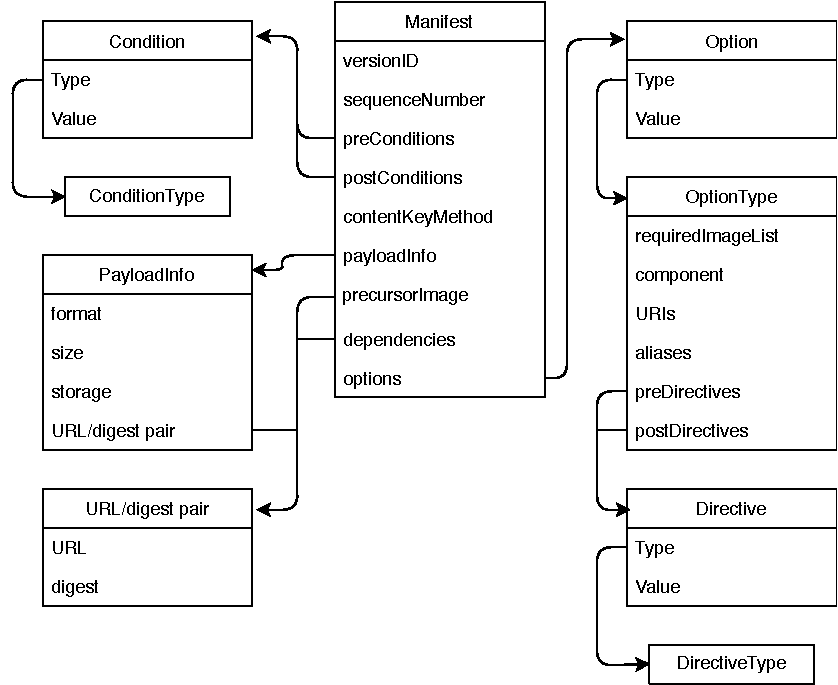
\includegraphics{images/manifest-format.pdf}
\end{figure}

Some of these elements are singular elements such as version ID and sequence number, they
are simply numbers that are bound to some upper size depending on packet structure. Their
sizes are deterministic and they are easy to parse. Other elements, for instance payload
information and conditions, have dynamic sizes. This is because the amount of information
needed for one update can differ quite drastically from another update. One update without
dependencies that is targeted for one specific class of device with no optional elements
can be described in a very small manifest. This small manifest would have no precursors,
dependencies, or options. The payload information would contain just one URI/digest pair,
and there are only two conditions, one vendor ID and one class ID.

Another update that is specifying differential updates for a wide class of devices will
need to specify much more information in the manifest. There will be several class IDs as
several classes are targeted. The different classes might not be running the same versions
of software or firmware and thus several dependencies are listed. Furthermore since
devices might not be able to reach the same servers, the manifest contains a list of
alises for the image, causing the manifest to contain many URI/digest pairs. This manifest
will be larger than the previous one described and the fields of this manifest will have
much different sizes. The dynamic nature of certain elements must be considered when
implementing the manifest as the packet structure must be prepared for it. 

The condition type, directive type, and option type structures provides flexibility to
implementers. The manifest format as it is specifies the optional elements of SUIT as
option types as well as vendor ID and class ID for condition type. It is easy to add new
types and thus add new conditions, options, or directives. The meaning of custom
conditions and directives are the same as the specified ones, conditions are either
parameters that must match some property of the device or invariants that must be true
before or after the update, and directives give instructions as how to unpack the update,
how to install it etc if so needed. The meaning of options though are completely dependant
on the specific option in mind, so new functionality can be embedded as an option. If the
current manifest format lacks some functionality for a specific deployment, an implementer
can add that piece of functionality in the form of an option, updating the server
preparing the manifest as well as the parser on the device.
Section~\ref{sec:manifest-implementation} discusses the manifest implementation used in
the thesis.
% TODO: Reference section where manifest implementation is shown

\section{Use Cases and Example Topologies}
\label{sec:use-cases-examples-topologies}
As discussed, operators, update servers, and devices can interact in many ways. The
architecture tries to be flexible allowing for different network topologies and
configurations. The important parts are that devices can enroll and register, all actors
have valid certificates, and that updates can be authorized. The following examples all
assume devices are enrolled and registered, and re-enrollment and updating profiles are
omitted to make the figures clearer.

Figure~\ref{fig:elderly-home} shows a use case where wearables of patients in an elderly
home need their operating system updated. A technician from the operating system vendor
assumes the role of an operator. The technician interacts with an authorization update
server and a dedicated update server to send the signed manifest and image with an
authorization token. The update server accepts the update and stores it for future use.
When the device is about to pull the update, it first requests an authorization token. The
authorization server does not handle the protocols used inside the constrained network and
thus the token request goes through a proxy on the edge of the network. After the device
has received the token, it pulls the signed manifest and image using the token to
authorize the pull.

\begin{figure}
    \caption{An operating system vendor technician updates patient wearable in an elderly home.}
    \label{fig:elderly-home}
    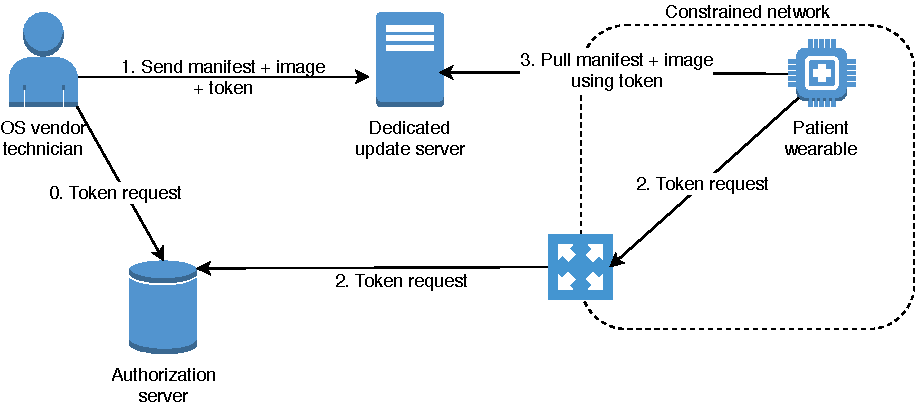
\includegraphics{images/use-case-elderly-home.pdf}
\end{figure}

In Figure~\ref{fig:smart-home} a technician from a smart light bulb vendor is updating a
light bulb controller in a smart home. The technician requests a token and sends it
together with the signed manifest and image to a home automation server living on the edge
of the constrained network. The server requests a token of its own and pushes the updates
to devices in its network. Both a light bulb controller, the intended target, and a
thermostat controller receives the update. The thermostat controller is supposed to only
accept updates from the thermostat vendor, thus the light bulb vendor technician is
unauthorized to perform this update. The thermostat controller rejects the update while
the light bulb controller accepts it and updates itself.

\begin{figure}
    \caption{A light bulb vendor technician updates a light bulb controller in a smart
                home, but the thermostat controller rejects it due to authorization
                issues.}
    \label{fig:smart-home}
    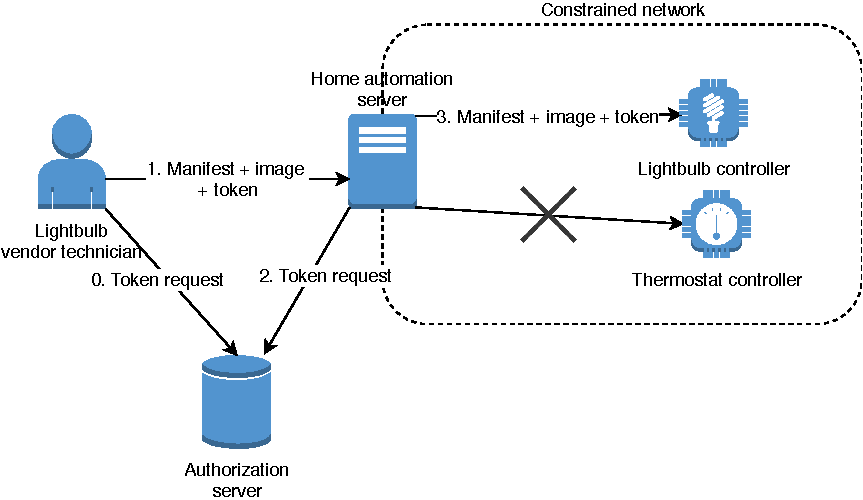
\includegraphics{images/use-case-smart-home.pdf}
\end{figure}

The last example shown in Figure~\ref{fig:industry} shows an on-site devops engineer
wanting to update a critical temperature sensor in an industry plant. The engineer first
requests a token to send the signed manifest directly to the device and a token to send
the signed image to the sensor update server. In this case, the update server is a more
capable IoT device in the constrained network. It needs to request an authorization token
to push the update to the device but is unable to speak the protocols used by the
authorization server. The update server instead goes through a proxy to send the token
request. With the token, the update can be sent to the device.

The device needs to authorize the token, but as it is a very constrained device it cannot
perform the necessary calculations. The device opts to perform an introspection request
through the proxy so the authorization server can help verifying the token. After the
device has received an answer, it can proceed applying the update.

\begin{figure}
    \caption{An on-site devops engineer updates a very constrained, critical temperature
                sensor in an industry plant. The constrained sensor asks for introspection
                data in order to verify the update server's token.}
    \label{fig:industry}
    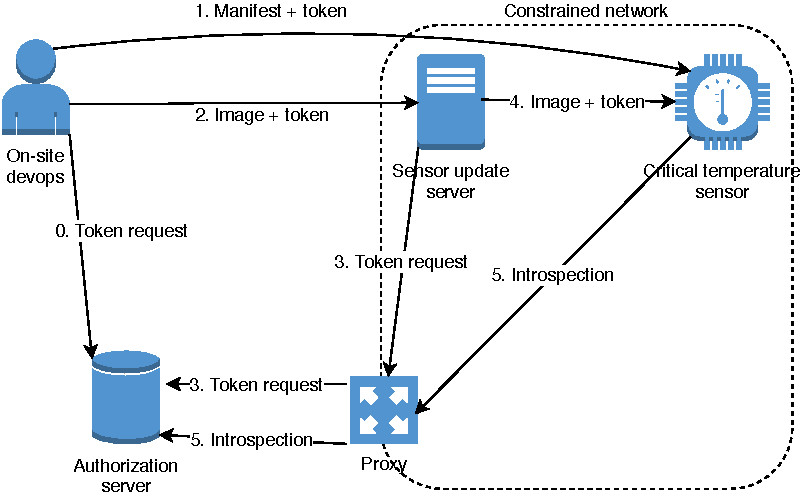
\includegraphics{images/use-case-industry.pdf}
\end{figure}

What these three examples have in common is that the operator always resides outside the
constrained network, devices always reside within the constrained network, and that
update servers transport updates to devices alongside authorization tokens. Since operators
reside in traditional networks using traditional protocols such as HTTP over TCP, a proxy
may be necessary to communicate with the often UDP based constrained networks. The update
server can act as a proxy, or a dedicated proxy could be used. If the operator has the
proper protocols implemented, they can communicate manifests directly to a device.

\end{document}